\documentclass[12pt,a4paper]{article}
\usepackage{graphicx}
\usepackage{wrapfig}

\title{Praktikum Physik - Beugung}
\author{Simon Marti, Patricia Schwab, Mirco Kocher}
\date{16.03.2012}

\parindent=0pt 
\begin{document}
\maketitle

%%
% Ziel
%%
\section*{Ziel}
Bestimmung der Gitterkonstanten mit dem Mikroskop und anhand der Beugungsmaxima von Helium und Wasserstoff.

%%
% Motivation
%%
\section*{Motivation}
Durch die Beleuchtung einse Gitters mit der Gr\"ossenordnung von $\sim$ 500 nm gelangt bei der Beugung Licht an Orte, wo es nach den Gesetzen der geometrischen Optik nicht hingelangen kann. Licht mit Strahlung verschiedener Wellenl\"angen von einer Gasentladungsr\"ohre werden in seine spektralen Komponenten aufgespalten. Die Emission der entsprechenden Lichtquanten wird bestimmten \"Uberg\"angen der Elektronen im Atom zugeordnet.


%%
% Theorie
%%
\section*{Theorie}
Der Beugungswinkel am Gitter ist durch folgende Formel gegeben
\begin{equation}\label{eq:g}
sin\varphi = n\cdot \frac{\lambda}{g}
\end{equation}

Die Frequenz beim Elektronensprung l\"asst sich folgendermassen bestimmen
\begin{equation}\label{eq:e}
\nu_{nm} = R\cdot \left(\frac{1}{m^2}-\frac{1}{n^2}\right) [\mbox{Hz}]
\end{equation}

Die Frequenz ist gegeben durch 
\begin{equation}\label{eq:f}
\nu = \frac{c}{\lambda} [\mbox{Hz}]
\end{equation}

%%
% Experiment 1
%%
\section*{Experiment I}
% Aufbau und Ablauf
\subsection*{Aufbau und Ablauf}
Mit einem Mikroskop wird ein optisches Gitter betrachtet und die Gitterkonstante durch abz\"ahlen bestimmt.

% Rohdaten
\subsection*{Rohdaten}
Anzahl Gitterlinien in einer Einheit des Mikroskops: 12 $\pm$ 0.5

Gr\"osse dieser Einheit: 0.0208mm

% Auswertung
\subsection*{Auswertung}
$g$ = (1.73$\cdot 10^{-6} \pm 0.069\cdot 10^{-6})$m

%%
% Experiment 2
%%
\section*{Experiment II}

% Aufbau und Ablauf
\subsection*{Aufbau und Ablauf}
\begin{center}
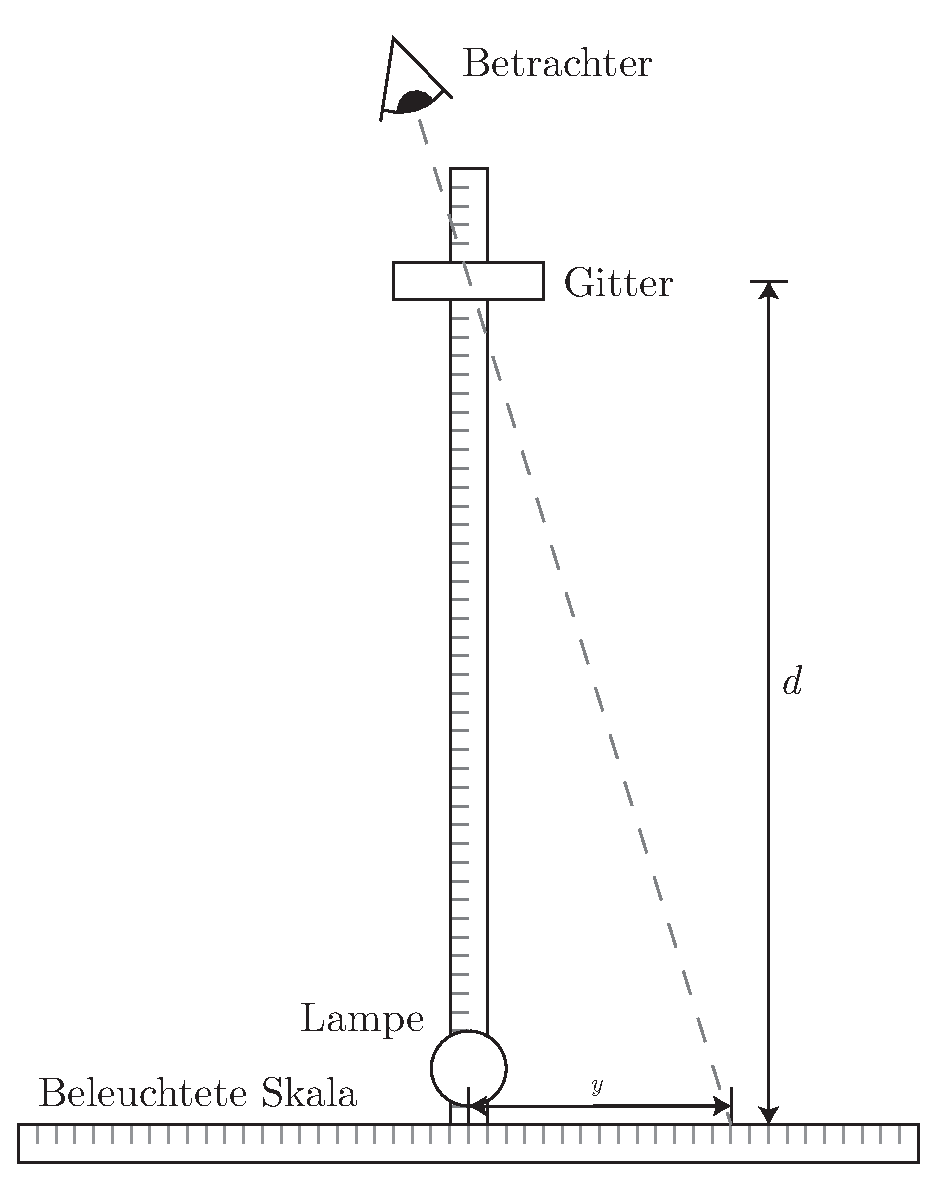
\includegraphics[width=13cm]{illustration.pdf}
\end{center}

Eine Heliumlampe wird auf einer Schiene direkt vor eine senkrecht zu Schiene stehende, beleuchtete Skala montiert. Etwas entfernt von der Lampe wird auf der Schiene ein optisches Gitter so montiert, dass ein Betrachter durch das Gitter die Lampe und dahinter die Skala sehen kann.

Der Betrachter (Simon) sieht nun durch das Gitter auf die Skala und sollte darauf mehrere farbige Beugungslinien sehen. Um die Abstand $y$ der Linien besser bestimmen zu k\"onnen f\"ahrt ein Gehilfe (Mirco) mit der Spitze eines Kugelschreibers \"uber die Skala bis sich diese mit einer der Beugungslinien \"uberlagert, was der Betrachter bekannt gibt. Da sich die Position der Beugungslinien je nach Blickwinkel des Betrachters ver\"andern kann wird jeweils der minimale und der maximale Abstand gemessen der gerade noch sichtbar ist. Aus den gemessenen Abst\"anden $y$ kann nun die Gitterkonstante nach Formel \ref{eq:g} ausgerechnet werden.

% Rohdaten
\subsection*{Rohdaten}
\begin{tabular}{|l|l|l|}
\hline
$\lambda$ [\AA]&$y_{min} [cm]$&$y_{max} [cm]$\\
\hline
7065&22.1&22.7\\
6678&23.7&24.6\\
5875&25.1&25.7\\
5015&25.8&26.5\\
4921&30.7&31.7\\
4713&36.1&37.4\\
4471&38.7&40.0\\
\hline
\end{tabular}\vspace{10pt}

Abstand $d$ = (80 $\pm$ 0.05)cm

% Auswertung
\subsection*{Auswertung}
Die Gitterkonstante $g$ kann durch umformen der Formel \ref{eq:g} berechnet werden:
\[ g = \frac{\lambda}{sin(tan^{-1}(\frac{y}{d}))} \]

\begin{tabular}{|l|l|}
\hline
$\lambda$ [\AA]&g [m]\\
\hline
7065&$1.6582\cdot 10^{-6}$\\
6678&$1.63083\cdot 10^{-6}$\\
5875&$1.62617\cdot 10^{-6}$\\
5015&$1.61411\cdot 10^{-6}$\\
4921&$1.61692\cdot 10^{-6}$\\
4713&$1.59976\cdot 10^{-6}$\\
4471&$1.60069\cdot 10^{-6}$\\
\hline
\end{tabular}\vspace{10pt}

Ausgehend von einem Fehler $s_y$ von 0.1cm:.\vspace{5pt}

$\overline{g} = (1.6210\cdot 10^{-6} \pm 0.0009\cdot 10^{-6})$m

%%
% Experiment 3
%%
\section*{Experiment III}

% Aufbau und Ablauf
\subsection*{Aufbau und Ablauf}
Im Aufbau von Experiment II wird die Heliumlampe durch eine Wasserstofflampe ersetzt und erneut der Abstand $y$ der Beugungslinien gemessen. Die einzigen beiden sichtbaren Beugungslinien die in diesem Versuch sind blau und rot.

Aus den beiden Abst\"anden $y$ wird die Wellenl\"ange der jeweiligen Farbe der Beugungslinien berechnet und daraus kann dann bestimmt werden durch welche Elektronenspr\"unge diese erzeugt worden sind.

% Rohdaten
\subsection*{Rohdaten}
\subsubsection*{Rot}
$y_{min}$ = (34.6 $\pm$ 0.1)cm

$y_{max}$ = (35.4 $\pm$ 0.1)cm

\subsubsection*{Blau}
$y_{min}$ = (24.5 $\pm$ 0.1)cm

$y_{max}$ = (25.4 $\pm$ 0.1)cm

% Auswertung
\subsection*{Auswertung}
Die Wellenl\"ange der beiden Beugungsmaxima k\"onnen nach Formel \ref{eq:g} unter Verwendung der Gitterkonstante aus Experiment I bestimmt werden.\vspace{5pt}

$\lambda_{rot}$ = (6722 $\pm$ 158)\AA

$\lambda_{blau}$ = (4994 $\pm$ 158)\AA

\vspace{5pt}
Die jeweiligen Frequenzen k\"onnen durch Formel \ref{eq:f} berechnet werden:\vspace{5pt}

$\nu_{rot}$ = (4.44788$\cdot 10^{14} \pm 9.486 \cdot 10^6$)Hz

$\nu_{blau}$ = (5.9879$\cdot 10^{14} \pm 9.486 \cdot 10^6$)Hz

\vspace{5pt}
Nach Formel \ref{eq:e} entsprechen die beiden Frequenzen ungef\"ahr den ersten beiden Spr\"ungen der Balmer-Serie:\vspace{5pt}

$\nu_{23} = 4.5667\cdot 10^{14}$Hz $\approx\nu_{rot}$

$\nu_{24} = 6.165\cdot 10^{14}$Hz $\approx\nu_{blau}$


%%
% Diskussion
%%
\section*{Diskussion}


\end{document}